\documentclass{sigchi}

% Use this section to set the ACM copyright statement (e.g. for
% preprints).  Consult the conference website for the camera-ready
% copyright statement.

% Copyright

%\setcopyright{acmcopyright}
%\setcopyright{rightsretained}
%\setcopyright{usgov}
%\setcopyright{usgovmixed}
%\setcopyright{cagov}
%\setcopyright{cagovmixed}
% DOI
\doi{https://doi.org/10.1145/3313831.XXXXXXX}
% ISBN
\isbn{978-1-4503-6708-0/20/04}
%Conference
\conferenceinfo{CHI'20,}{April  25--30, 2020, Honolulu, HI, USA}
%Price
\acmPrice{\$15.00}

% Use this command to override the default ACM copyright statement
% (e.g. for preprints).  Consult the conference website for the
% camera-ready copyright statement.

%% HOW TO OVERRIDE THE DEFAULT COPYRIGHT STRIP --
%% Please note you need to make sure the copy for your specific
%% license is used here!
% \toappear{
% Permission to make digital or hard copies of all or part of this work
% for personal or classroom use is granted without fee provided that
% copies are not made or distributed for profit or commercial advantage
% and that copies bear this notice and the full citation on the first
% page. Copyrights for components of this work owned by others than ACM
% must be honored. Abstracting with credit is permitted. To copy
% otherwise, or republish, to post on servers or to redistribute to
% lists, requires prior specific permission and/or a fee. Request
% permissions from \href{mailto:Permissions@acm.org}{Permissions@acm.org}. \\
% \emph{CHI '16},  May 07--12, 2016, San Jose, CA, USA \\
% ACM xxx-x-xxxx-xxxx-x/xx/xx\ldots \$15.00 \\
% DOI: \url{http://dx.doi.org/xx.xxxx/xxxxxxx.xxxxxxx}
% }
\toappear{}

% Arabic page numbers for submission.  Remove this line to eliminate
% page numbers for the camera ready copy
% \pagenumbering{arabic}

% Load basic packages
\usepackage{balance}       % to better equalize the last page
\usepackage{graphics}      % for EPS, load graphicx instead 
\usepackage[T1]{fontenc}   % for umlauts and other diaeresis
\usepackage{txfonts}
\usepackage{mathptmx}
\usepackage[pdflang={en-US},pdftex]{hyperref}
\usepackage{color}
\usepackage{booktabs}
\usepackage{textcomp}

% Some optional stuff you might like/need.
\usepackage{microtype}        % Improved Tracking and Kerning
% \usepackage[all]{hypcap}    % Fixes bug in hyperref caption linking
\usepackage{ccicons}          % Cite your images correctly!
% \usepackage[utf8]{inputenc} % for a UTF8 editor only

% If you want to use todo notes, marginpars etc. during creation of
% your draft document, you have to enable the "chi_draft" option for
% the document class. To do this, change the very first line to:
% "\documentclass[chi_draft]{sigchi}". You can then place todo notes
% by using the "\todo{...}"  command. Make sure to disable the draft
% option again before submitting your final document.
\usepackage{todonotes}

% Paper metadata (use plain text, for PDF inclusion and later
% re-using, if desired).  Use \emtpyauthor when submitting for review
% so you remain anonymous.
\def\plaintitle{Preventing Bias in Machine Learning by using Bias Aware Algorithms: An Empirical Experimental Study - Full Report}
\def\plainauthor{First Author, Second Author, Third Author,
  Fourth Author, Fifth Author, Sixth Author}
\def\emptyauthor{}
\def\plainkeywords{Authors' choice; of terms; separated; by
  semicolons; include commas, within terms only; this section is required.}
\def\plaingeneralterms{Documentation, Standardization}

% llt: Define a global style for URLs, rather that the default one
\makeatletter
\def\url@leostyle{%
  \@ifundefined{selectfont}{
    \def\UrlFont{\sf}
  }{
    \def\UrlFont{\small\bf\ttfamily}
  }}
\makeatother
\urlstyle{leo}

% To make various LaTeX processors do the right thing with page size.
\def\pprw{8.5in}
\def\pprh{12in}
\special{papersize=\pprw,\pprh}
\setlength{\paperwidth}{\pprw}
\setlength{\paperheight}{\pprh}
\setlength{\pdfpagewidth}{\pprw}
\setlength{\pdfpageheight}{\pprh}

% Make sure hyperref comes last of your loaded packages, to give it a
% fighting chance of not being over-written, since its job is to
% redefine many LaTeX commands.
\definecolor{linkColor}{RGB}{6,125,233}
\hypersetup{%
  pdftitle={\plaintitle},
% Use \plainauthor for final version.
%  pdfauthor={\plainauthor},
  pdfauthor={\emptyauthor},
  pdfkeywords={\plainkeywords},
  pdfdisplaydoctitle=true, % For Accessibility
  bookmarksnumbered,
  pdfstartview={FitH},
  colorlinks,
  citecolor=black,
  filecolor=black,
  linkcolor=black,
  urlcolor=linkColor,
  breaklinks=true,
  hypertexnames=false
}

% create a shortcut to typeset table headings
% \newcommand\tabhead[1]{\small\textbf{#1}}

% End of preamble. Here it comes the document.
\begin{document}

\title{\plaintitle}

\numberofauthors{3}
\author{%
  \alignauthor{Andy Gray\\
    \affaddr{445348}\\
    \email{445348@swansea.ac.uk}}
}

\maketitle

\section{Introduction}

[Project Discription]\\
We aim to remove the potential gender bias in a suggested pay to an employee from data with a clear gender bias within the dataset. 

[Motivation]\\
\textbf{In 2018, women, no matter their background, on average earned just 82 cents for every \$1 earned by men \cite{1}. ML requires vast amounts of past data to inform future events, with AI and machine learning being the key driver behind many decisions. However, with there being a well-known gap between a person's gender and their pay, the ML models will only learn this and use this as a factor in their decisions making. Therefore, to stop this from happening, a system needs to be put into place to remove this process's bias.} 

\textbf{Using fairness techniques at preprocessing stages \cite{3} of supervised learning, we will aim to remove the bias of someone's gender from a suggested pay salary for an individual. } %Needs changing -> copy job from part 1.

[Summary of existing lit]\\

%blah blah blah blah blah blah blah blah blah blah blah blah blah blah blah blah blah blah

[Problems with lit]\\
	Mothers in part-time jobs are getting hit by a "pay penalty" and are often not given pay rises linked to experience \cite{bbc_mothers_suffering}. - due to working part-time and being on less?

	"More than three out of four UK companies pay their male staff more than their female staff, and in nine out of 17 sectors in the economy, men earn 10 per cent or more on average than women" \cite{gender_pay_FT}. - due to pay scales

	Therefore, even though by law in the UK, it is illegal to pay men and women different amounts for doing the same job, a gender pay gap still exists, and there is still a difference in equal pay. This difference in equal pay is driven by the use of salary pay scale ranges and, in some cases, a bias to think that women are not as valuable as men within a similar role.
	
	So we are proposing a solution that will help reduce the bias within salary negotiations that removes the elements of gender bias to produce a tool that will look at the person's job role and their years of experience. Therefore, not taking into account previous pay and if they were working full or part-time.

[Project Spec]\\ % Maybe not needed.
%blah blah blah blah blah blah blah blah blah blah blah blah blah blah blah blah blah blah

[Result findings]\\
%blah blah blah blah blah blah blah blah blah blah blah blah blah blah blah blah blah blah

[Overview]\\
	We will next look into the background of this topic and review existing literature. We will then explain the study design, the libraries used to create to solution and the dataset used, and the pre and post data processing techniques used. We will then present the results and analyse them. Finally, we will be discussing the over empirical study and concluding the overall findings.

\section{Background \& Literature Review}
	%Gender Pay Gap
	In 2018 companies with 250 or more employees were expected to file their first data on their gender pay gap data. With the actions of companies publishing their data, this created a significant discussion around what people earn and ultimately what difference in what men and women earn \cite{bbc_gender_pay_gap}. In 2017 a UK male earned 18.4\% more than a woman \cite{ons_gender_pay_gap_17}. 
	
	It is important to note that the pay gap is not the same thing as equal pay. Equal pay is a law that got brought in in 1970 that ensures that men and women doing the same job should get paid the same amount \cite{bbc_gender_pay_gap}. Due to the equal pay act 1970 \cite{equal_pay_act_1070} and the equality act 2010 \cite{equal_act_2010}, it is illegal to pay works different amounts for the same man if they are a man or woman.
	
	While companies like DDB UK, the legal entity, which includes Adam\&EveDDB, Tribal Worldwide, Gutenberg Global and Cain \& Abel, releases detailed gender pay gap reports each year. The company has, since 2017, enforced a rule that 50\% of the candidates for senior positions getting interviewed must be female. Additionally, they are initiating mandatory unconscious bias training \cite{uk_gender_gap}. However, while making these changes, a recent slowdown in reducing the gap has occurred. Additionally, the gender pay gap between graduates has not improved since 1993. There have been no improvements despite the gap getting a reduction for non-graduates \cite{bbc_mothers_suffering}.
	
	Mothers in part-time jobs are getting hit by a "pay penalty" and are often not given pay rises linked to experience \cite{bbc_mothers_suffering}.
	By the time a couple's first child is aged 20, many mothers earn nearly a third less than the fathers. A key factor was women working part-time in motherhood \cite{ifs_mothers_suffer}. This situation that mothers find themselves in gets referred to as the "motherhood penalty" \cite{tuc_motherhood}. For mothers born in 1970, there is a 34\% overall gender pay gap. This gap is primarily due to the impact of parenthood on earnings, with women earning less and men earning more after having children. However, there is a significant but much smaller gender pay gap between childless women and men born at this time, a 12\% gap \cite{tuc_motherhood}.
	
	
	In 2020, "More than three out of four UK companies pay their male staff more than their female staff, and in nine out of 17 sectors in the economy, men earn 10 per cent or more on average than women" \cite{gender_pay_FT}. This is an issue generated when workers get paid, on a scale, based on their "experience". It opens up an opportunity for employees to be paid different amounts based on what is perceived to be their worth, which can have an unconscious bias at the heart of it. % [As when people need to negotiate for their salaries men will think they are worth more than they actually are, while women will usually take the first offer]. 
	
	

\subsection{Study Design}
	Our study is around the topic of bias in algorithms and looking at ways to remove these biases. The study will be looking at ways to detect the bias, measure it and then reduce it. Our study got carried out in a manner that follows an empirical experimental study method. 

	Our study has looked into ways to identify bias within a dataset and then look at ways to remove this bias, ensuring that protected characteristics, in our case gender, do not impact or impede a person's proposed suggested salary.  

	We aimed to try and find out if there was first any bias within the dataset. We did this by first plotting out the dataset based on the characteristic of male and female. We initially created a model that would truthfully represent the gender bias within the model's predictions.

	To achieve removing the bias, we extracted the prediction-specific interactions. By getting the interactions, we could cancel out their effect and the influence driven by the gender variable. We then re-calculate our predictions, which immediately shows the removal of any sign of prejudice within the dataset. Additionally, the model conscientiously captures the variation driven by the employee's years of employment and career path. 

	This bias-aware approach to modelling can be applied to other forms of input types, with a similar approach being used by Google \cite{google_ref}

\subsection{Libraries}
	We used Python 3 \cite{python} to create the empirical experiment. Additional libraries used were Pandas \cite{pandas} to allow us to load in the data and wrangle the data frames. Seaborn \cite{seaborn} was also used to visualise the data. XGBoost \cite{xgboost} to create the model and extract the critical interactions from within the model. 

\subsection{Dataset and Data Pre \& Post-processing}
	We create our dataset to simulate data containing gender, years of experience, and career type. Our overall aim is to predict the salary of someone while taking these features into account. The type of career will be focusing on software engineering (SWE) and consulting.  We decided to create this dataset synthetically due to time restrictions and lack of data collection containing real-world figures of these two career options. Most datasets found provided more of an overview than the exact figures, and we believe this is due to the sensitive and personal nature of the required data.
	
	We based the synthesised data on general assumptions about pay. There will be a clear positive relationship between years of experience and a person's salary. An SWE will earn less than a consultant, and being male will earn them more money than females generally. Additional factors within the data are that in SWE roles, women will start at the lower end of the scale while men will be varied and, therefore, women will be over time increasing their pay. However, this increase will be at a faster rate than men but from a lower starting point. While for consulting, both males and females will start at the same rate, but men will get more considerable increases in pay over time compared to their women counterparts. 
	
	%[data preprocessing]\\
	As some of the columns contained text categorical data types, we first processed the data to convert this to a numerical value. The data got split into a train test set of 70/30\%. 
	
	%[data postprocessing]\\
	We ensured that when the model was making its predictions, the predictions' interactions got provided with the results. We then created a bias variable based on the model's gender values and a bias index based on the values being in the datasets feature names and the bias-variance. 
	
	We were then able to create a de-biased $\hat{y}$ value by summing the interaction values and then minus 1. The outputted value then has created the new values with the gender bias removed.


	%Synthetic dataset based around two job types -> why because was hard to find data set that does not provide "just an overview". 

	%pandas.get\_dummies

\subsection{Parameter Settings}
	We set the learning rate to the model as 0.1, between the range of 0 and 1 that the model expects. The learning task for the model got set to regression squared error, which looks at the regression squared loss. The number of boost rounds got set to 100 as well.

\section{Results \& Analysis}
	
	When we look at the dataset in its original representation (see fig: \ref{fig:original_data}), we can see a clear divide between the male and female pay salaries. We can see that the regression line for SWE is \textasciitilde{42,000} for women and \textasciitilde{60,000} for men starting, and then both these gender values increase to \textasciitilde{105,000}. Therefore both values roughly reaching the same value at 20 years of experience. While for consulting, the starting off values are very close to each other, \textasciitilde{60-65,000}. However, these values completely deviate when at the top end of the scale. Men have a value of \textasciitilde{115,000}, while women have a value of \textasciitilde{105,000}.

	\begin{figure}[h]
		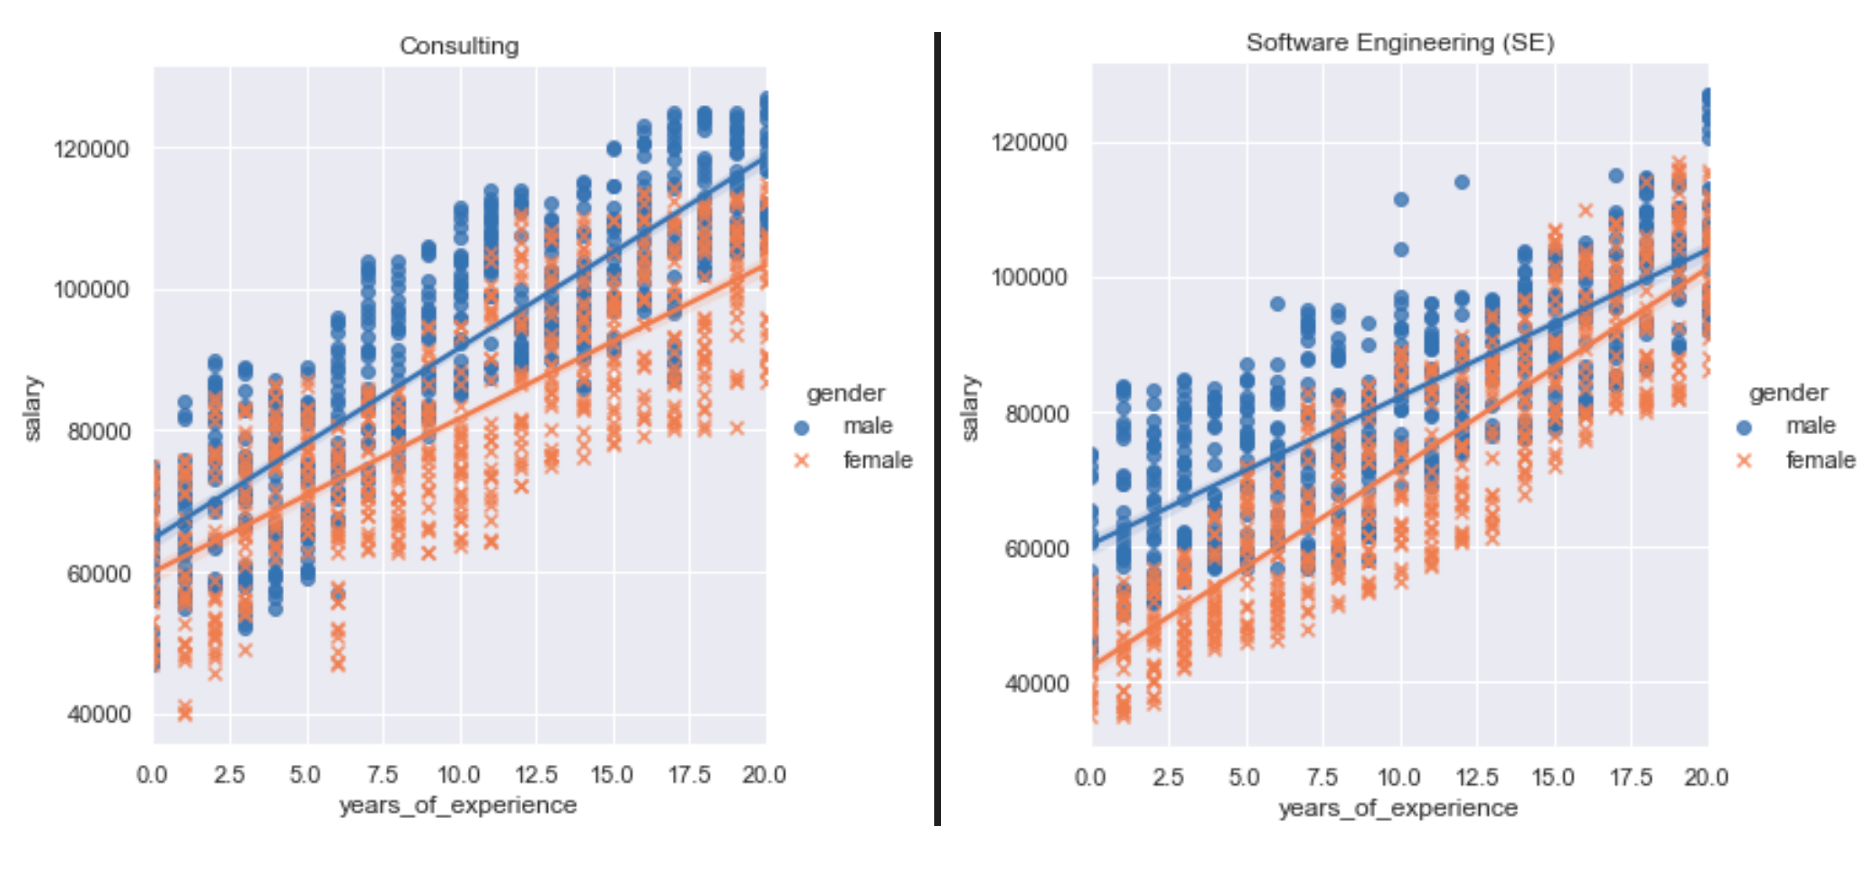
\includegraphics[width=9.2cm]{original_data.png}
		\caption{The dataset's datapoints and initial regression fit with the data being unmodified, split by gender and career option.}
		\label{fig:original_data}
		\centering
	\end{figure}

	Before removing the gender bias, we can see that the model's predictions mirror a similar result to the original data's general trend for SWE (see fig: \ref{fig:se_comparison}).  However, when we look at the values when the gender bias gets removed, the model's predictions almost align perfectly with each other. It is evident that there is some difference between the two gender predictions, but the difference is extremely marginal when concerning SWE employees. With both men and women being \textasciitilde{65,000} starting and \textasciitilde{112,000} at 20 years of experience.
	
	\begin{figure}[h]
		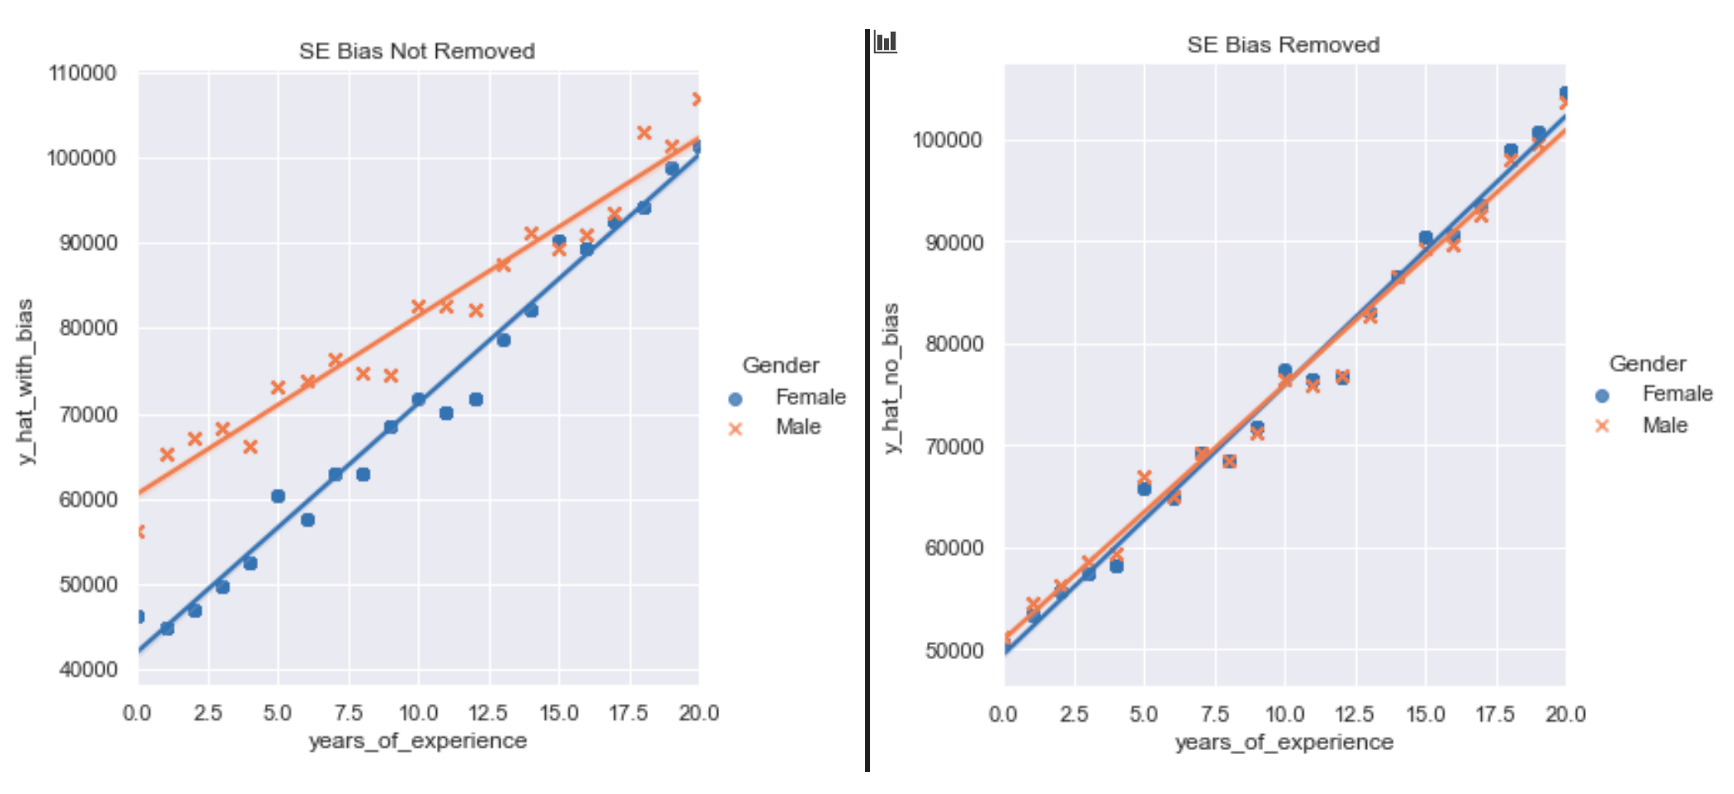
\includegraphics[width=9.2cm]{se_comparison.png}
		\caption{The model's 'Software Engineering' initial $\hat{y}$ regression prediction with bias and the $\hat{y}$ predition after the bias has been removed.}
		\label{fig:se_comparison}
		\centering
	\end{figure}

	In relations to consulting, we can see that the predictions with the bias still intact, the model's predictions follow the same patterns as the data overall (see fig: \ref{fig:consulting_comparison}).  The regression representation is close to being equally matched. With the starting off wage for both men and women around \textasciitilde{60-65,000} and the top end of the range being \textasciitilde{109-111,000}. It is evident that there is some difference between the two gender predictions, but the difference is very marginal concerning consulting employees. 

	\begin{figure}[h]
		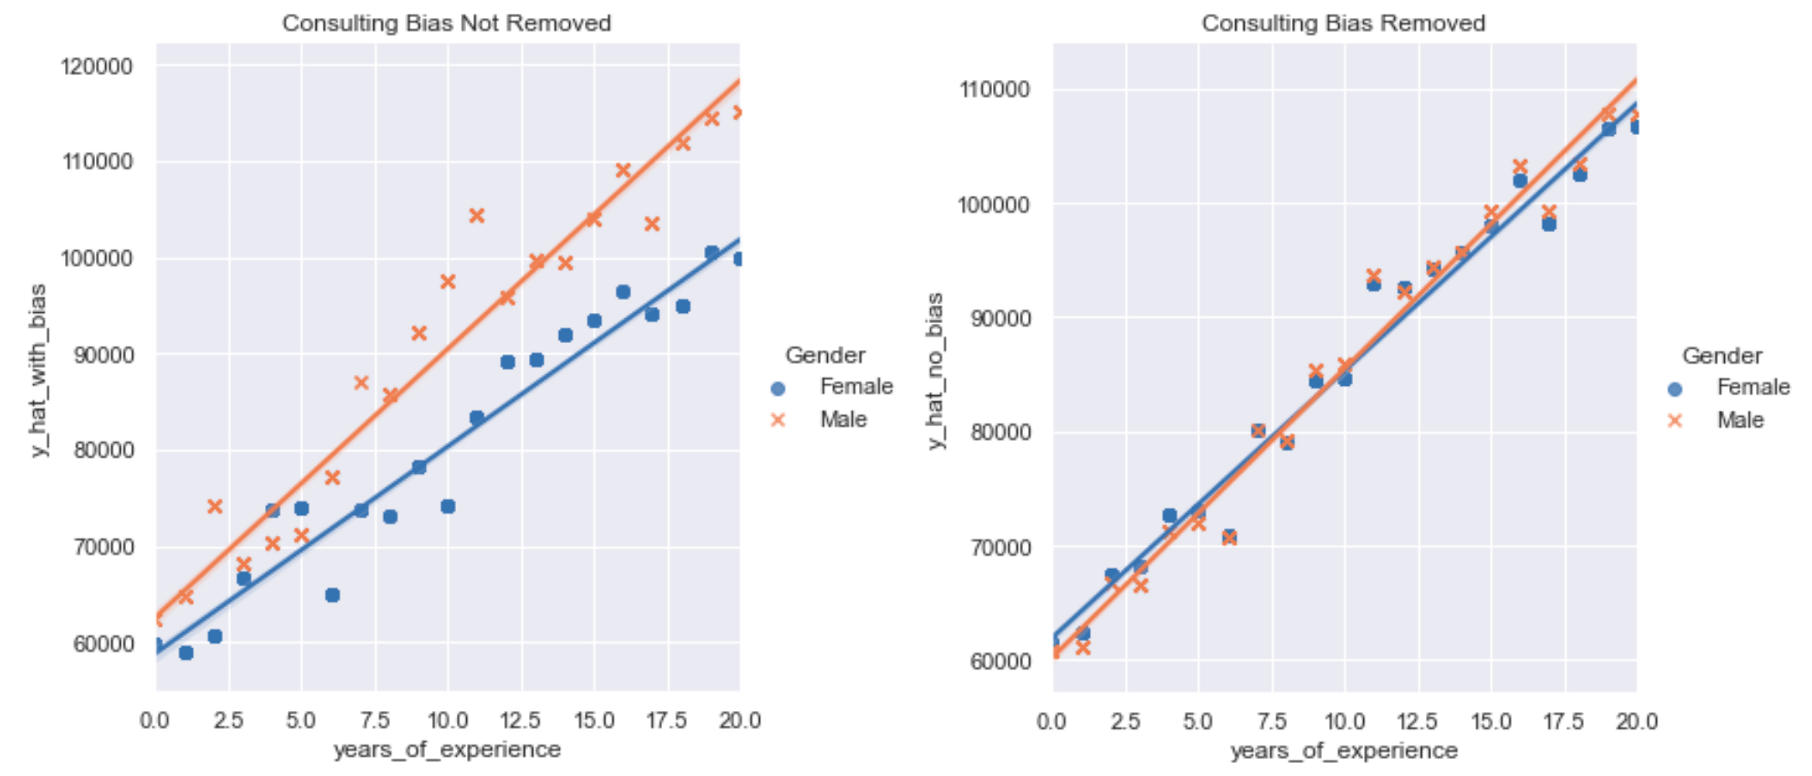
\includegraphics[width=9.2cm]{consulting_comparison.png}
		\caption{The model's 'Consulting' initial $\hat{y}$ regression prediction with bias and the $\hat{y}$ predition after the bias has been removed.}
		\label{fig:consulting_comparison}
		\centering
	\end{figure}

	Therefore, overall we can see that the approach has created almost perfect un-bias results between genders over the different career options. While it has not matched the values up entirely between the genders, it has created a much more even representation than prior. 

	% Maybe add in RMSPE and other metrics in as well possibly?

\section{Discussion \& Conclusion}
	[discussion]
	
	[conclusion] \\
	\textbf{I would like to point out from the outset that there is no question that this approach will lead to a decrease in model performance on your validation data. In our contrived example, the RMSPE is 12\% for predictions that encode bias and 14\% for predictions where we removed the gender contribution. Nonetheless, this decrease in performance is acceptable and encouraged in many settings. After all, the purpose of your models is not only to make good predictions but to also allow you to identify ways to pull levers, such as modify user behavior on your website or prevent harmful things from happening when diagnosing a disease. Hence, if you want to build a model that is not prejudiced by your data, you can’t go wrong with letting the model first measure the amount of prejudice and then resetting all the bias contributing factors to zero.}


\newpage
% BALANCE COLUMNS
\balance{}
% REFERENCES FORMAT
% References must be the same font size as other body text.
\bibliographystyle{SIGCHI-Reference-Format}
\bibliography{sample}

\end{document}

%%% Local Variables:
%%% mode: latex
%%% TeX-master: t
%%% End:
